\section{Technical Description}
As a starting point for the implementation, the work by \cite{gallego_2023} has been kindly taken as reference. In order to better follow the changes here pointed out, it is recommended to first refer to that work.

The main changes performed on the implementation of the strategy are the following.

\begin{itemize}
    \item \textbf{Position sizing}: In the original work, once the trigger was activated, the positions were opened with the position size determined on the day of the trigger change. That position was then kept until the position was determined to be closed. In the new position sizing, the position is also entered on the moment the trigger is activated but it is changed daily in accordance with the daily changes in position sizes as calculated in equation \eqref{e:position-sizes}. This allows for, on the one hand, better performance as the dynamic position sizing better follows the specification of the position sizing model in equations \eqref{e:position-size-model-1} amd \eqref{e:position-size-model-2} better adjusting to changes in implied volatilty and price changes. On the other hand, this also allows for calculating the position sizes in a vectorized way from the trigger vector, making the position sizing calculation process faster and more efficient. 
    \item \textbf{Return calculation}: In the original implementation returns for each timestep were calculated as a sum of the returns of the long and short positions. This was changed to first consider the full portfolio equation \textcolor{red}{REFERENCE PORTFOLIO EQUATION} taking into account the returns of the cash position -- positive or negative -- as the long and short positions are hardly ever completely self financed. The return calculation function was also extended in order to extract the long and short returns sepparately from the overall returns. 
    \item \textbf{Spread option $\Delta$}: The calculation of the d1 as per \eqref{e:calc-d1} was modified in order to remove the risk free rate from the numerator and to remove an absolute value on the difference between logprices. 
    \item \textbf{Trigger}: The trading trigger was modified to fit exactly equation \eqref{e:trigger-1}. This was also a simpler and faster implementation than the previous trigger. 
    \item \textbf{Win rate}: An in-built counter has been implemented to measure what percentage of the positions end up yielding returns higher than the risk free rate for the period in which they are traded. This win rate is calculated for overall returns, long returns and short returns. 
    \item \textbf{Active positions}: Similarly to the win rate, an in-built counter has been implemented to measure the number of pairs which are being actively traded on any given day.  
    \item \textbf{Pairs considered}: Since the cointegration estimator and the position sizing methods assumes which asset of the pair is long and which is short, the set of pairs considered for trading has been extended to enable both assets to be either long or short in all pairs. 
    \item \textbf{Process batching}: In order to enable to strategy to be run on a much larger universe of assets, the parameter estimation process and the return calculation process for all pairs has been divided into batches. After a given batch of pair's parameters are estimated, they are saved as a pickle file. The joint returns of that set of pairs are calculated and again saved to permanent memory as a pickle file, after the returns of pairs in which the trigger was not activated for the whole period are erased to reduce the unnecessary use of memory. The variables containing all pair parameters and return calculations are erased from RAM and the next batch of pairs can be calculated. If the process crashes, it does not have to restart from the beginning as the batches which have already finished have been saved and don't need to be calculated again. After all batches have been calculated, all saved sets of returns are read into memory and aggreagated, yielding the final set of strategy returns, which can be then finally saved for later analysis. This batching process had to be implemented as the CPU did not have enough memory to hold all the variables for the parameter estimation process or the return calculation process for all pairs, even though most of the calculations were already performed in parallel in the original implementation and thus the variables were reused reducing the memory footprint. The memory profiling of the program before the changed was implemented can be seen in \autoref{fig:memory-profile}.
    \begin{figure}[ht]
        \centering
        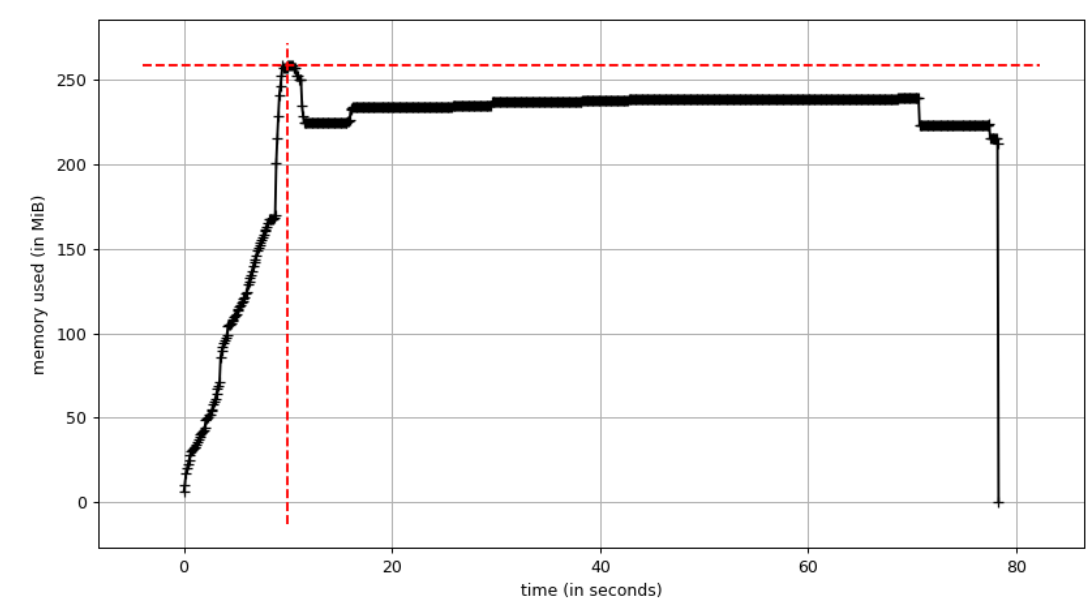
\includegraphics[width=300px]{assets/memory-profile.png}
        \caption{Memory profile of execution before introduction of batching}
        \label{fig:memory-profile}
    \end{figure}
\end{itemize}